% \section{Моделирование старения ГС}
% \subsection{Алгоритм моделирования старения ГС}
% \begin{figure}[h]
%   \centering
%   \includegraphics[width=0.7\linewidth]{assets/AlgDegrEc}
%   \caption{Блок схема алгорит моделирования старения ГС}
%   \label{img:AlgDegrEc}
% \end{figure}

% \subsection{Результат моделирования}
% \begin{figure}[h]
%   \centering
%   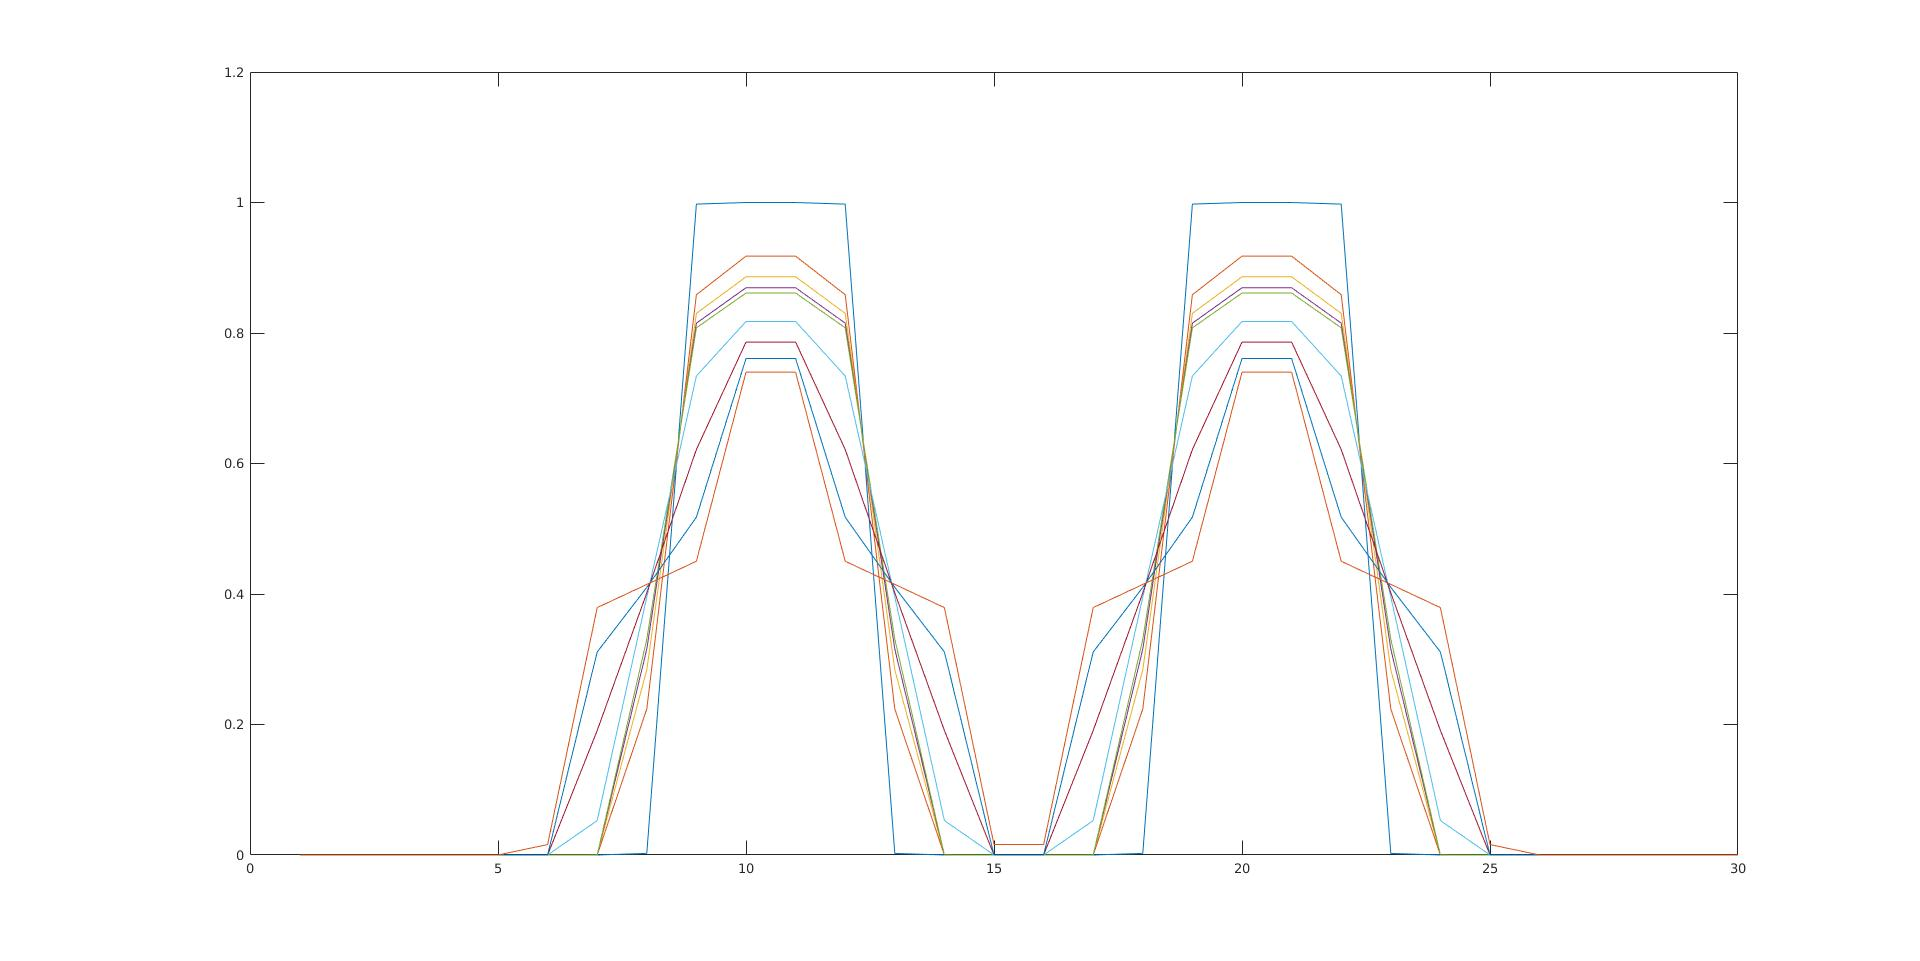
\includegraphics[width=1.1\linewidth]{assets/AlX10}
%   \caption{Результат моделирования старения}
%   \label{img:AlX10}
% \end{figure}

\section{Моделирование диффузионного размытия в <<открытой системе>> $i\!-\!GaAs/i\!-\!Al_{45}Ga_{55}As$}
\begin{figure}[h]
  \centering
  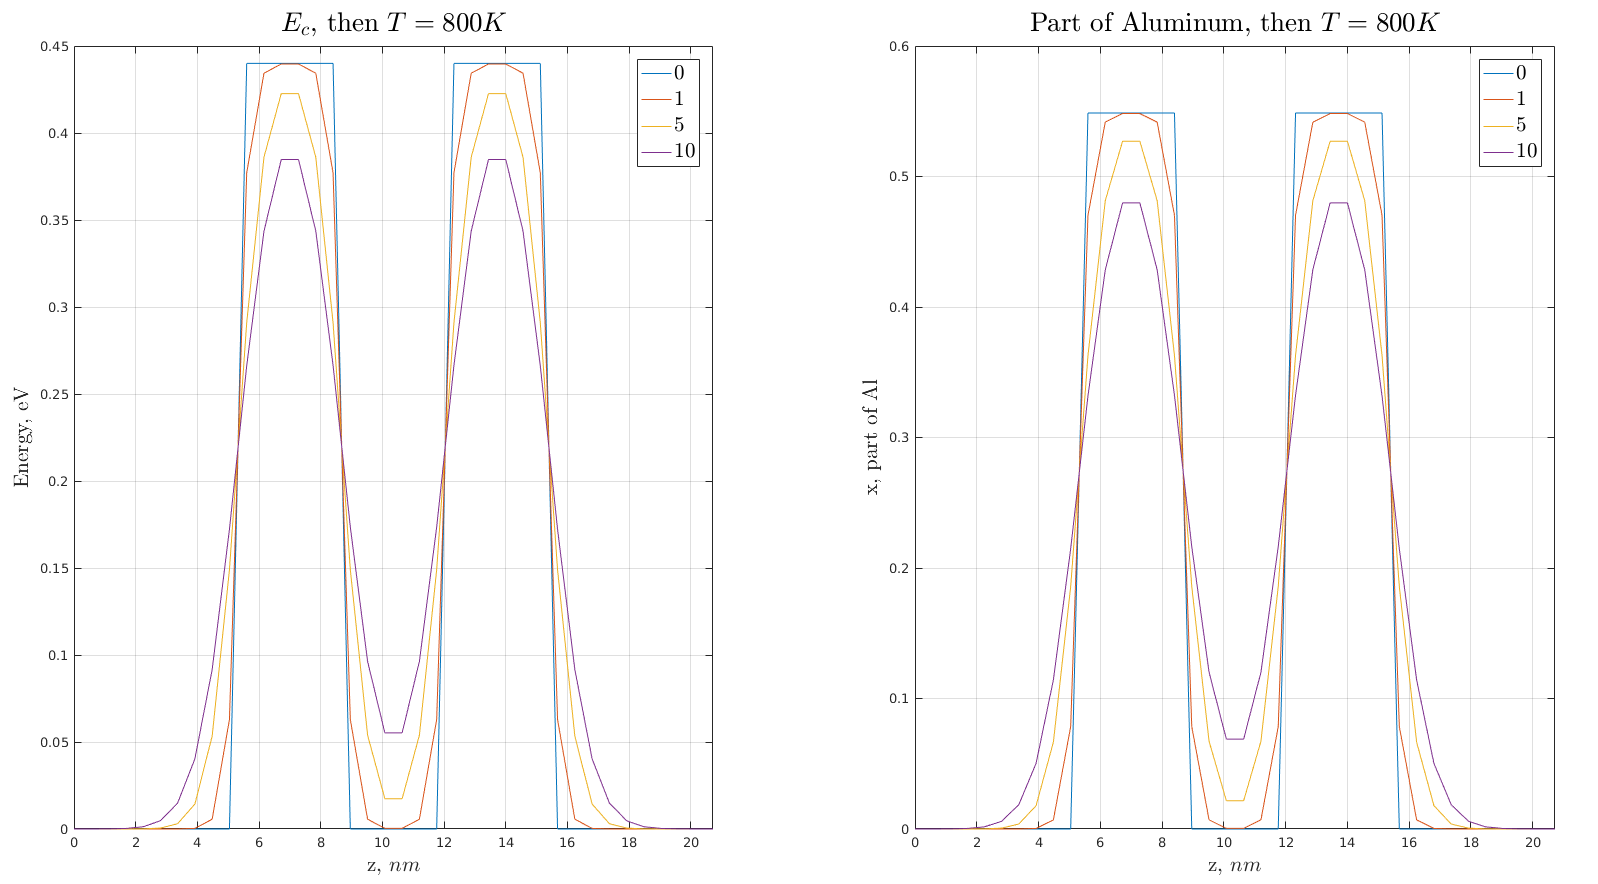
\includegraphics[width=0.9\linewidth]{DOAlGaAs}
  \caption{Диффузионное размытие}
\end{figure}

\begin{figure}[h]
  \centering
  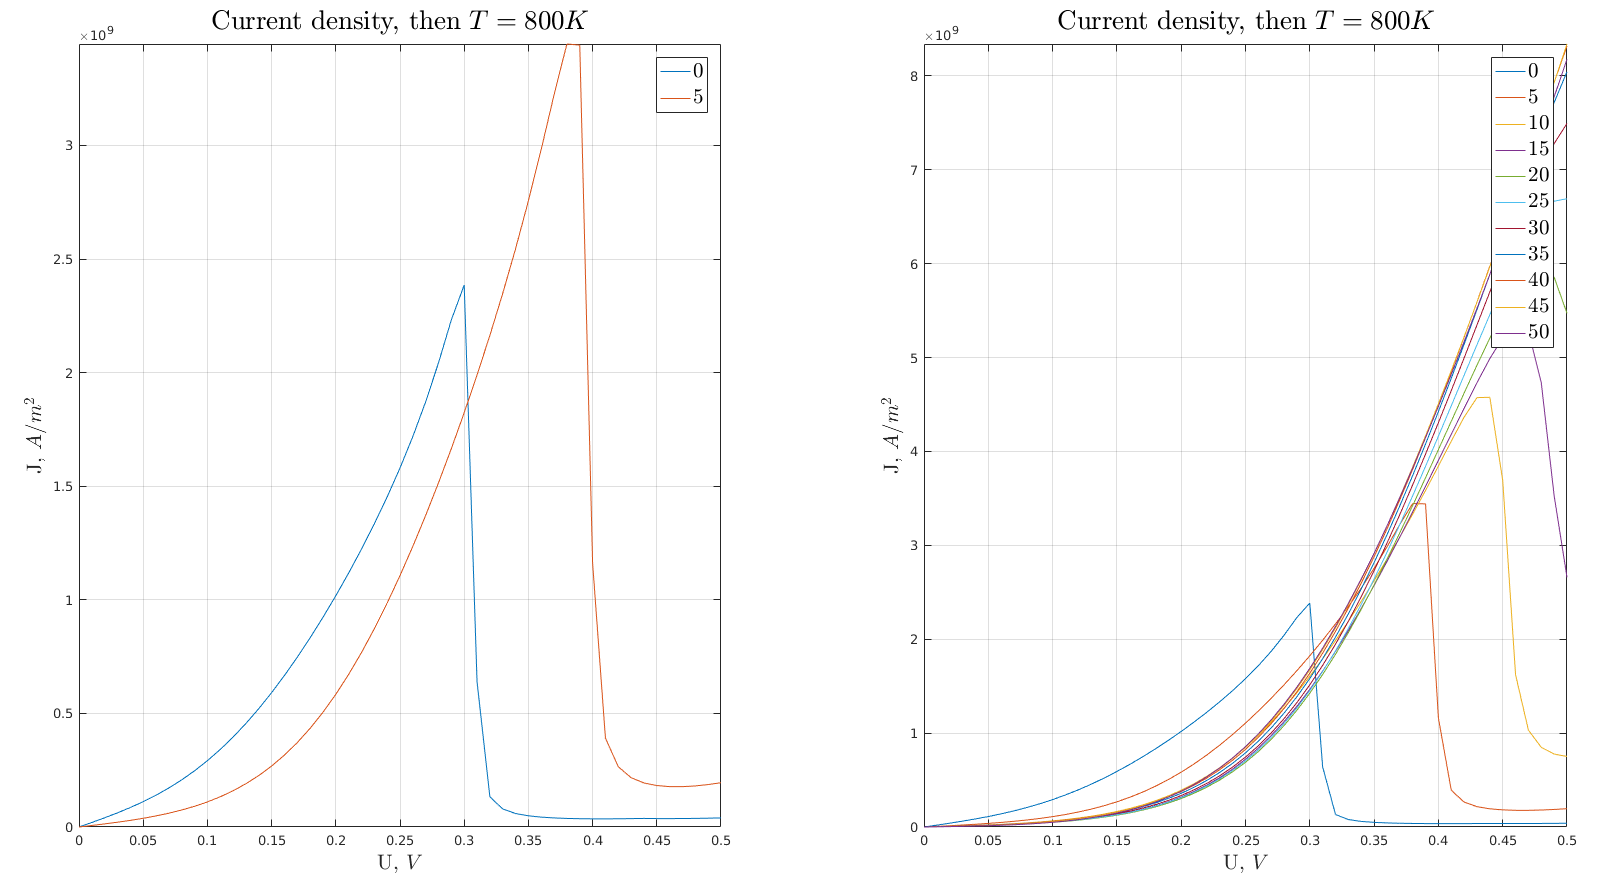
\includegraphics[width=0.9\linewidth]{JDOAlGaAs}
  \caption{Деградация ВАХ}
\end{figure}

\begin{figure}[h]
  \centering
  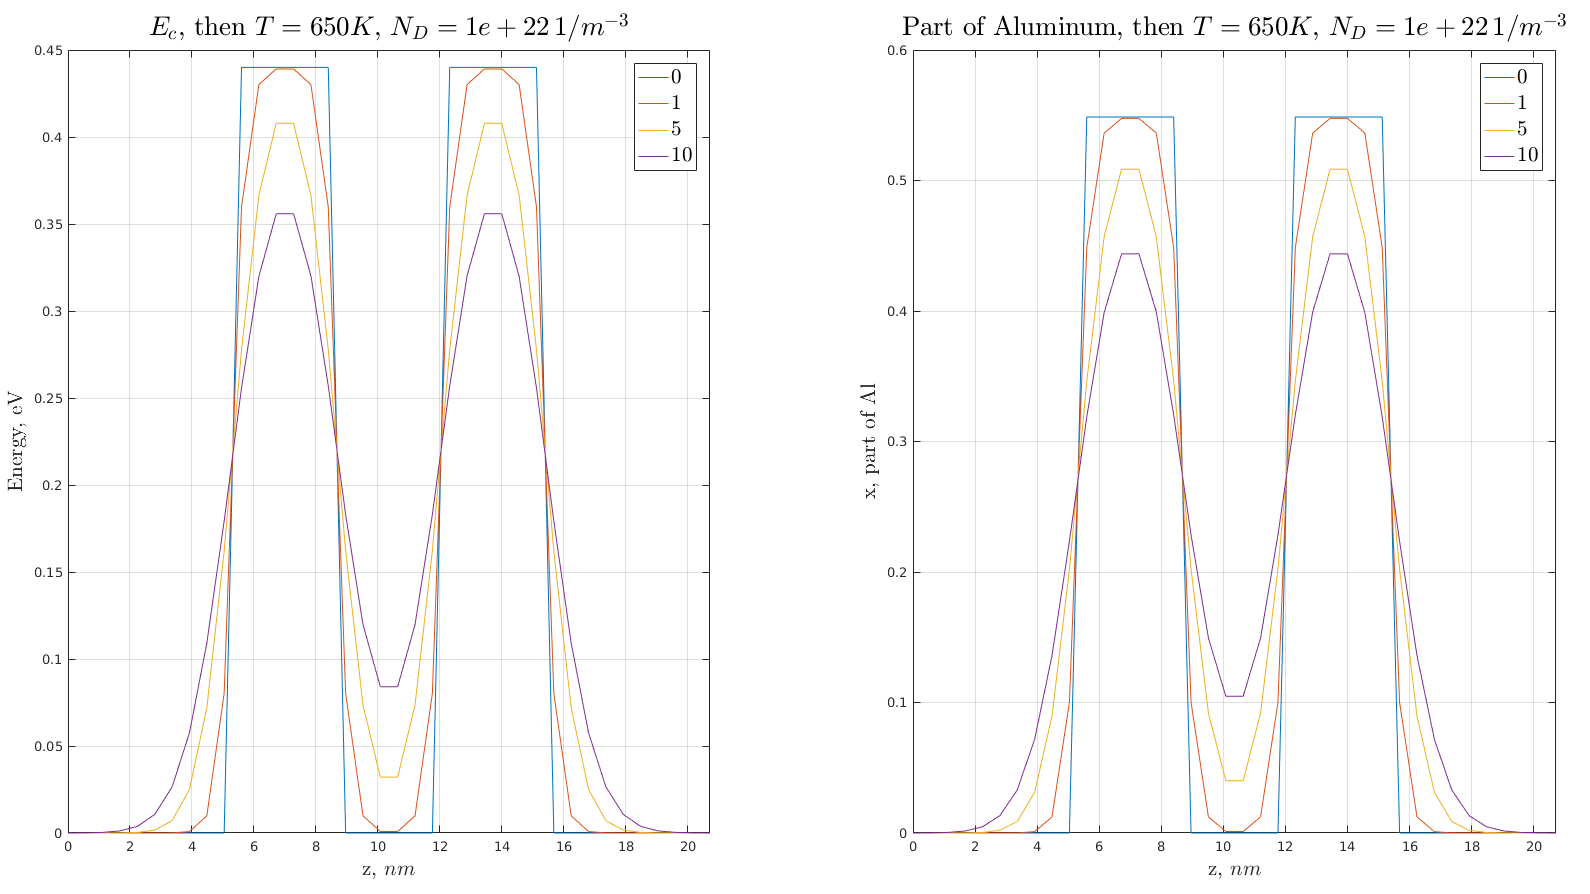
\includegraphics[width=\linewidth]{DOAlGaAsNd}
  \caption{Диффузионное размытие с учетом примеси, $Nd = 5*10^{15}sm^{-3}$}
\end{figure}

\begin{figure}[h]
  \centering
  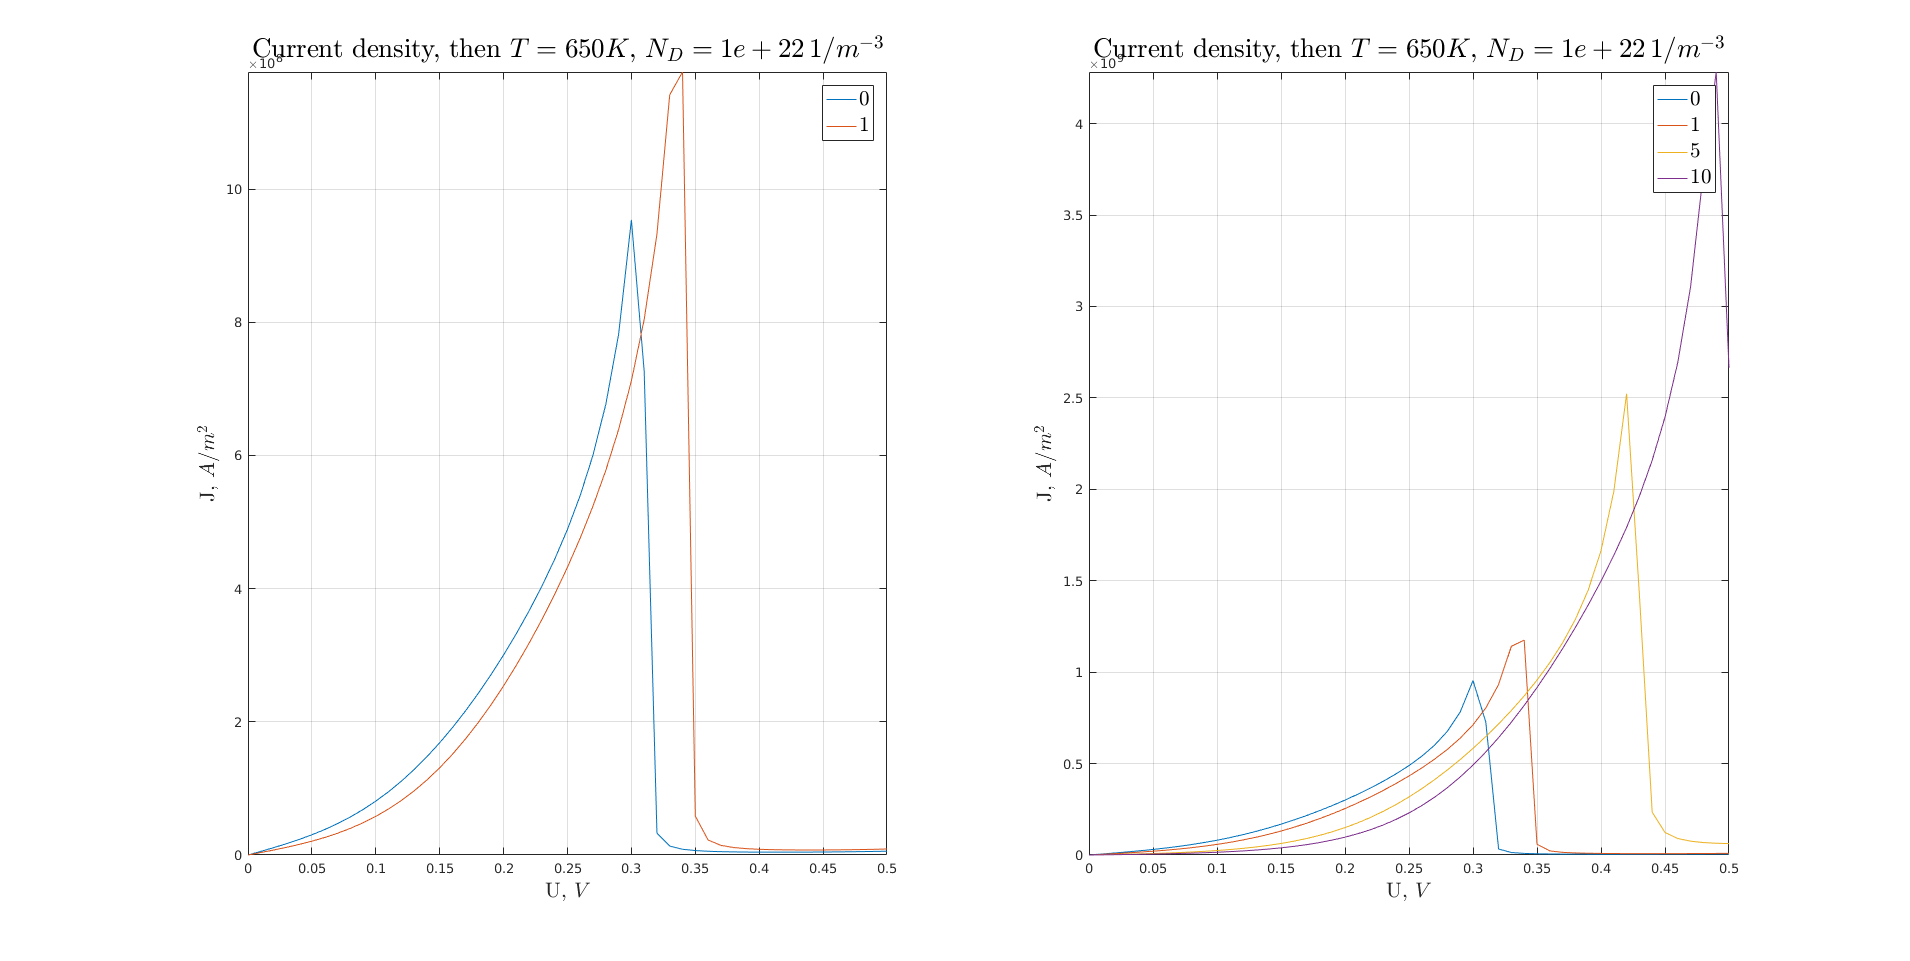
\includegraphics[width=\linewidth]{JDOAlGaAsNd}
  \caption{Деградация ВАХ с учетом примеси, $Nd = 5*10^{15}sm^{-3}$}
\end{figure}